% Options for packages loaded elsewhere
\PassOptionsToPackage{unicode}{hyperref}
\PassOptionsToPackage{hyphens}{url}
%
\documentclass[
  english,
  man, donotrepeattitle,floatsintext]{apa7}
\title{Data irregularities across five implicit learning articles: Comments on Lola, Tzetzis, and Zetou (2012); Lola and Tzetzis (2020); Lola and Tzetzis (2021); Tzetzis and Lola (2010); Tzetzis and Lola (2015)}
\author{Brad McKay\textsuperscript{1} \& Michael J. Carter\textsuperscript{1}}
\date{}

\usepackage{amsmath,amssymb}
\usepackage{lmodern}
\usepackage{iftex}
\ifPDFTeX
  \usepackage[T1]{fontenc}
  \usepackage[utf8]{inputenc}
  \usepackage{textcomp} % provide euro and other symbols
\else % if luatex or xetex
  \usepackage{unicode-math}
  \defaultfontfeatures{Scale=MatchLowercase}
  \defaultfontfeatures[\rmfamily]{Ligatures=TeX,Scale=1}
\fi
% Use upquote if available, for straight quotes in verbatim environments
\IfFileExists{upquote.sty}{\usepackage{upquote}}{}
\IfFileExists{microtype.sty}{% use microtype if available
  \usepackage[]{microtype}
  \UseMicrotypeSet[protrusion]{basicmath} % disable protrusion for tt fonts
}{}
\makeatletter
\@ifundefined{KOMAClassName}{% if non-KOMA class
  \IfFileExists{parskip.sty}{%
    \usepackage{parskip}
  }{% else
    \setlength{\parindent}{0pt}
    \setlength{\parskip}{6pt plus 2pt minus 1pt}}
}{% if KOMA class
  \KOMAoptions{parskip=half}}
\makeatother
\usepackage{xcolor}
\IfFileExists{xurl.sty}{\usepackage{xurl}}{} % add URL line breaks if available
\IfFileExists{bookmark.sty}{\usepackage{bookmark}}{\usepackage{hyperref}}
\hypersetup{
  pdftitle={Data irregularities across five implicit learning articles: Comments on Lola, Tzetzis, and Zetou (2012); Lola and Tzetzis (2020); Lola and Tzetzis (2021); Tzetzis and Lola (2010); Tzetzis and Lola (2015)},
  pdfauthor={Brad McKay1 \& Michael J. Carter1},
  pdflang={en-EN},
  pdfkeywords={Meta-science; GRIMMER; Effect sizes; Perceptual motor learning},
  hidelinks,
  pdfcreator={LaTeX via pandoc}}
\urlstyle{same} % disable monospaced font for URLs
\usepackage{graphicx}
\makeatletter
\def\maxwidth{\ifdim\Gin@nat@width>\linewidth\linewidth\else\Gin@nat@width\fi}
\def\maxheight{\ifdim\Gin@nat@height>\textheight\textheight\else\Gin@nat@height\fi}
\makeatother
% Scale images if necessary, so that they will not overflow the page
% margins by default, and it is still possible to overwrite the defaults
% using explicit options in \includegraphics[width, height, ...]{}
\setkeys{Gin}{width=\maxwidth,height=\maxheight,keepaspectratio}
% Set default figure placement to htbp
\makeatletter
\def\fps@figure{htbp}
\makeatother
\setlength{\emergencystretch}{3em} % prevent overfull lines
\providecommand{\tightlist}{%
  \setlength{\itemsep}{0pt}\setlength{\parskip}{0pt}}
\setcounter{secnumdepth}{-\maxdimen} % remove section numbering
% Make \paragraph and \subparagraph free-standing
\ifx\paragraph\undefined\else
  \let\oldparagraph\paragraph
  \renewcommand{\paragraph}[1]{\oldparagraph{#1}\mbox{}}
\fi
\ifx\subparagraph\undefined\else
  \let\oldsubparagraph\subparagraph
  \renewcommand{\subparagraph}[1]{\oldsubparagraph{#1}\mbox{}}
\fi
\newlength{\cslhangindent}
\setlength{\cslhangindent}{1.5em}
\newlength{\csllabelwidth}
\setlength{\csllabelwidth}{3em}
\newlength{\cslentryspacingunit} % times entry-spacing
\setlength{\cslentryspacingunit}{\parskip}
\newenvironment{CSLReferences}[2] % #1 hanging-ident, #2 entry spacing
 {% don't indent paragraphs
  \setlength{\parindent}{0pt}
  % turn on hanging indent if param 1 is 1
  \ifodd #1
  \let\oldpar\par
  \def\par{\hangindent=\cslhangindent\oldpar}
  \fi
  % set entry spacing
  \setlength{\parskip}{#2\cslentryspacingunit}
 }%
 {}
\usepackage{calc}
\newcommand{\CSLBlock}[1]{#1\hfill\break}
\newcommand{\CSLLeftMargin}[1]{\parbox[t]{\csllabelwidth}{#1}}
\newcommand{\CSLRightInline}[1]{\parbox[t]{\linewidth - \csllabelwidth}{#1}\break}
\newcommand{\CSLIndent}[1]{\hspace{\cslhangindent}#1}
% Manuscript styling
\usepackage{upgreek}
\captionsetup{font=singlespacing,justification=justified}

% Table formatting
\usepackage{longtable}
\usepackage{lscape}
% \usepackage[counterclockwise]{rotating}   % Landscape page setup for large tables
\usepackage{multirow}		% Table styling
\usepackage{tabularx}		% Control Column width
\usepackage[flushleft]{threeparttable}	% Allows for three part tables with a specified notes section
\usepackage{threeparttablex}            % Lets threeparttable work with longtable

% Create new environments so endfloat can handle them
% \newenvironment{ltable}
%   {\begin{landscape}\begin{center}\begin{threeparttable}}
%   {\end{threeparttable}\end{center}\end{landscape}}
\newenvironment{lltable}{\begin{landscape}\begin{center}\begin{ThreePartTable}}{\end{ThreePartTable}\end{center}\end{landscape}}

% Enables adjusting longtable caption width to table width
% Solution found at http://golatex.de/longtable-mit-caption-so-breit-wie-die-tabelle-t15767.html
\makeatletter
\newcommand\LastLTentrywidth{1em}
\newlength\longtablewidth
\setlength{\longtablewidth}{1in}
\newcommand{\getlongtablewidth}{\begingroup \ifcsname LT@\roman{LT@tables}\endcsname \global\longtablewidth=0pt \renewcommand{\LT@entry}[2]{\global\advance\longtablewidth by ##2\relax\gdef\LastLTentrywidth{##2}}\@nameuse{LT@\roman{LT@tables}} \fi \endgroup}

% \setlength{\parindent}{0.5in}
% \setlength{\parskip}{0pt plus 0pt minus 0pt}

% Overwrite redefinition of paragraph and subparagraph by the default LaTeX template
% See https://github.com/crsh/papaja/issues/292
\makeatletter
\renewcommand{\paragraph}{\@startsection{paragraph}{4}{\parindent}%
  {0\baselineskip \@plus 0.2ex \@minus 0.2ex}%
  {-1em}%
  {\normalfont\normalsize\bfseries\itshape\typesectitle}}

\renewcommand{\subparagraph}[1]{\@startsection{subparagraph}{5}{1em}%
  {0\baselineskip \@plus 0.2ex \@minus 0.2ex}%
  {-\z@\relax}%
  {\normalfont\normalsize\itshape\hspace{\parindent}{#1}\textit{\addperi}}{\relax}}
\makeatother

% \usepackage{etoolbox}
\makeatletter
\patchcmd{\HyOrg@maketitle}
  {\section{\normalfont\normalsize\abstractname}}
  {\section*{\normalfont\normalsize\abstractname}}
  {}{\typeout{Failed to patch abstract.}}
\patchcmd{\HyOrg@maketitle}
  {\section{\protect\normalfont{\@title}}}
  {\section*{\protect\normalfont{\@title}}}
  {}{\typeout{Failed to patch title.}}
\makeatother
\shorttitle{Commentary on Lola \& Tzetzis papers}
\keywords{Meta-science; GRIMMER; Effect sizes; Perceptual motor learning}
\usepackage{lineno}

\linenumbers
\usepackage{csquotes}
\usepackage{pdflscape}
\usepackage{xcolor}
\raggedbottom
\pagewiselinenumbers
\ifXeTeX
  % Load polyglossia as late as possible: uses bidi with RTL langages (e.g. Hebrew, Arabic)
  \usepackage{polyglossia}
  \setmainlanguage[]{english}
\else
  \usepackage[main=english]{babel}
% get rid of language-specific shorthands (see #6817):
\let\LanguageShortHands\languageshorthands
\def\languageshorthands#1{}
\fi
\ifLuaTeX
  \usepackage{selnolig}  % disable illegal ligatures
\fi


\authornote{

\addORCIDlink{Brad McKay}{0000-0002-7408-2323}

\addORCIDlink{Michael J. Carter}{0000-0002-0675-4271}

Correspondence concerning this article should be addressed to Brad McKay, 1280 Main Street West, Ivor Wynne Centre Room AB-131 A1, McMaster University, Hamilton ON Canada, L8S 4K1. E-mail: \href{mailto:bradmckay8@gmail.com}{\nolinkurl{bradmckay8@gmail.com}}

}

\affiliation{\vspace{0.5cm}\textsuperscript{1} Department of Kinesiology, McMaster University}

\abstract{
We present a critical re-analysis of five implicit learning papers published by the same authors between 2010 and 2021. We calculated effect sizes for each pairwise comparison reported in the papers using the data published in each article. We further identified mathematically impossible data reported in multiple papers, either with deductive logic or by conducting a GRIMMER analysis of reported means and standard deviations. We found the pairwise effect sizes were implausible in all five articles in question, with Cohen's \emph{d} values often exceeding 100 and sometimes exceeding 1000. Impossible statistics were reported in four out of the five articles. Reported test statistics and \(\eta^{2}\) values were also implausible, with several \(\eta^{2}\) = .99 and even \(\eta^{2}\) = 1.0 for between-subjects main effects. The results reported in the five articles in question are unreliable. Many of the problems we identified could be spotted without further analysis, highlighting the need for adequate statistical training in the field of motor learning.
}



\begin{document}
\maketitle

Statistical reporting errors may commonly occur in psychology articles (Brown \& Heathers, 2017; Nuijten, Hartgerink, van Assen, Epskamp, \& Wicherts, 2016) and such errors are often consistent with hypothesized results (Bakker \& Wicherts, 2011). When the primary conclusions in research articles depend on reporting errors, replicability is unlikely and future research may be wasted if researchers attempt to build on the erroneously reported results (Munafò et al., 2017). In this paper, we scrutinize five papers published by the same two authors\footnote{One of the five papers had a third author.}, where the authors report a high number of erroneous or implausible data on which their primary conclusions depend. We first became aware of the Lola and Tzetzis (2021) paper when the paper was highlighted in a social media post (Gray, 2021). During an initial read through by one of us (BM), a number of reporting and/or statistical issues were noticed. The paper also referenced past research published by these authors. Given our cause for concern over the issues found in the Lola and Tzetzis (2021) paper, we deemed it necessary to examine these other papers. We remain agnostic to the sources of error in each of these papers. Nevertheless, the data irregularities we found are similar across the target articles and at times even include repeated values (e.g., \(F\)-statistics) across multiple papers. Regardless of the conclusion one reaches with respect to the mechanism behind these errors, it is our contention that the results reported in these papers are unreliable and that the respective journals in which the papers are published should take corrective actions. Below, we outline our causes for concern and the overarching issues we found across the five articles in question.

\hypertarget{the-articles-in-question}{%
\subsection{The Articles in Question}\label{the-articles-in-question}}

We reanalyzed five articles by Afroditi Lola, George Tzetzis, and their colleague (Lola \& Tzetzis, 2020, 2021; Lola et al., 2012; Tzetzis \& Lola, 2010, 2015). All five papers described experiments that sampled young females who were enrolled in a volleyball camp (see Table \ref{tab:table1}). In their experiments, the authors investigated the effects of implicit and explicit instructions on learning motor and perceptual skills. Our reanalysis of the target articles evaluated the plausibility of the reported means, standard deviations, and test statistics. We will refer to the five articles throughout this paper using the following numbering system:

\begin{enumerate}
\def\labelenumi{\arabic{enumi}.}
\item
  Lola, A.C., \& Tzetzis, G.C. (2021). The effect of explicit, implicit and analogy instruction on decision making skill for novices, under stress. \emph{International Journal of Sport and Exercise Psychology}, 1-21. \url{https://doi.org/10.1080/1612197X.2021.1877325}
\item
  Lola, A.C., \& Tzetzis, G.C. (2020). Analogy versus explicit and implicit learning of a volleyball skill for novices: The effect on motor performance and self-efficacy. \emph{Journal of Physical Education and Sport}, 20(5), 2478-2486. \url{https://doi.org/10.7752/jpes.2020.05339}
\item
  Tzetzis, G.C., \& Lola, A.C. (2015). The effect of analogy, implicit, and explicit learning on anticipation in volleyball serving. \emph{International Journal of Sport Psychology}, 46(2), 152-166. \url{https://doi.org/10.7352/IJSP.2015.46.152}
\item
  Lola, A.C., \& Tzetzis, G.C., \& Zetou, H. (2012). The effect of implicit and explicit practice in the development of decision making in volleyball serving. \emph{Perceptual and Motor Skills}, 114(2), 665-678. \url{https://doi.org/10.2466/05.23.25.PMS.114.2.665-678}
\item
  Tzetzis, G.C., \& Lola, C.A. (2010). The role of implicit, explicit instruction and their combination in learning anticipation skill, under normal and stress conditions. \emph{International Journal of Sport Sciences and Physical Education}, 1, 54-59.\footnote{This article is in a journal of a publishing group that has been identified as a potential predatory journal. Further, we were unable to find an archived version of this article on the journal's webpage and were only able to find a posted version on ResearchGate (\url{https://www.researchgate.net/publication/341001393_THE_ROLE_OF_IMPLICIT_EXPLICIT_INSTRUCTION_AND_THEIR_COMBINATION_IN_LEARNING_ANTICIPATION_SKILL_UNDER_NORMAL_AND_STRESS_CONDITIONS}). In fact, the earliest available issue on the journal's webpage is from 2016.}
\end{enumerate}

\begin{table}

\caption{\label{tab:table1}Participant demographics in each of the target articles.}
\fontsize{11}{13}\selectfont
\begin{threeparttable}
\begin{tabular}[t]{ll}
\toprule
Target article & Sample size and participant details\\
\midrule
\addlinespace[0.3em]
\multicolumn{2}{l}{\textbf{Article 1}}\\
\hspace{1em}Lola \& Tzetzis (2021) & 60 females, age range: 10 to 11 years ($M_{age}$ = 10.48, SD = 0.911)\textsuperscript{a}\\
\addlinespace[0.3em]
\multicolumn{2}{l}{\textbf{Article 2}}\\
\hspace{1em}Lola \& Tzetzis (2020) & 80 females, age range: 10 to 11 years ($M_{age}$ = 10.48, SD = 0.911)\textsuperscript{a}\\
\addlinespace[0.3em]
\multicolumn{2}{l}{\textbf{Article 3}}\\
\hspace{1em}Tzetzis \& Lola (2015) & 60 females, age range: 9 to 12 years ($M_{age}$ = 10.48, SD = 0.91)\textsuperscript{a}\\
\addlinespace[0.3em]
\multicolumn{2}{l}{\textbf{Article 4}}\\
\hspace{1em}Lola et al (2012) & 60 females, age range: 10 to 12 years ($M_{age}$ = 11.2, SD = 0.3)\\
\addlinespace[0.3em]
\multicolumn{2}{l}{\textbf{Article 5}}\\
\hspace{1em}Tzetzis \& Lola (2010) & 48 females, age range: 12 to 13 years ($M_{age}$ = 12.38, SD = 0.34)\\
\bottomrule
\end{tabular}
\begin{tablenotes}
\item \textit{Note.} 
\item[a] Articles 1-3 report identical means and standard deviations for the age of their participants despite a different sample size in Article 2 from Articles 1 and 3, and a different age range in Article 3 from Articles 1 and 2.
\end{tablenotes}
\end{threeparttable}
\end{table}

Although there were some differences between the reported experiments in the target articles, there were many methodological commonalities that can be summarized. All five articles involved female children learning a volleyball skill as part of a volleyball camp. In each case, the participants were reported to have minimal experience (i.e., were described as novices) with the task at hand. The purpose of all five experiments was to evaluate perceptual or motor learning differences as a function of the type of instruction received during practice. Each experiment included a pre-test, an acquisition (i.e., practice) phase involving 12 sessions spaced over four weeks, and a post-test. The authors also included a high stress test in Articles 1 and 5.

In Articles 1-3, the groups differed with respect to the type of instruction received: implicit, explicit, or analogy. In Articles 4 and 5, a sequential group (see below for description) replaced the analogy group. All five experiments also included a control group that did not practice the task. Implicit instruction did not contain any explicit information for how to perform the task and the learners were asked to perform a distracting task like counting backwards while practicing to prevent them from acquiring declarative rules for performance. In contrast, explicit instruction consisted of direct verbal instructions for performing the task. Analogy instruction was considered a type of implicit instruction wherein an analogy or metaphor was provided to the learner. For example, ``Imagine that the opponents' surface is covered with water. Send the ball where there is more water and no opponents at the court.'' (Lola \& Tzetzis, 2021, p. 9). Sequential instruction involved receiving explicit instruction for the first half of training followed by implicit instruction for the second half of training. Across experiments, the authors predicted that implicit forms of instruction---implicit, analogy, and sequential---would be more effective than explicit instruction for motor and perceptual learning. This advantage was also predicted to be greater when testing was conducted in a high stress situation. In Lola and Tzetzis (2021) for instance, high stress was induced by falsely telling participants that the best performers would be selected for a draft to the national team. Further, it was predicted that analogy or sequential instruction would offer improvements relative to implicit instruction.

The primary outcome measures used in these experiments were reaction time (Articles 1, 3, 4, and 5), response accuracy (Articles 1, 3, 4), and motor performance measured on a 4-point scale (Article 2). In addition, Articles 1 and 5 included a measure of state anxiety, the Competitive State Anxiety Inventory-2 (Tsorbatzoudis, Barkoukis, Kaissidis-Rodafinos, \& Grouios, 1998), and Article 2 had a measure of self-efficacy using a Likert scale. Articles 1, 3, 4, and 5 also analyzed the number of explicit rules recalled.

\hypertarget{methods}{%
\section{Methods}\label{methods}}

None of the five articles in question included a link to a public repository where the data could be accessed. We first wrote (email sent February 10, 2021) the corresponding author for Article 1 and asked if they would be willing to share the data for this experiment. The authors' response was that the data could not be shared as they were not finished with their analyses and were in the process of running different tests (A. Lola, personal communication, February 12 2021). We followed up this email (sent February 12 2021) by asking whether they would instead be willing to share the data from Articles 2-5 as these articles were less recent and presumably, all planned analyses had been completed. After a 2 week period with no response, we followed up with a third email (sent February 26 2021) and reiterated our interest in obtaining their data from Articles 2-5. The authors' response was that they were unable to share data from any of these articles because in some cases they no longer had the data and in other cases they had plans to conduct further analyses (A. Lola, personal communication, March 2 2021).

Our first two requests did not include any indication about our concerns regarding the data irregularities. Subsequently, in a fourth email (sent April 12 2021) we outlined our concerns for each article and once again reiterated our request to the authors to share any available data for any of the target articles. These requests were once again refused. The authors did address some specific concerns regarding Article 1, but for the most part only provided more general responses to our concerns. Interestingly, parts of their responses were inaccurate relative to information in the target articles---increasing our concerns about these articles. The authors did admit that some of the values reported in the target articles were incorrect but did not identify which values or articles. Despite this, the authors maintained that the data irregularities---identified in our email and described in this paper---do not impact the veracity of their analyses or conclusions (A. Lola, personal communication, April 22 2021). We illustrate below that the data \emph{and} analyses reported in each of the articles reviewed are unreliable. Our extracted data and analysis scripts can be accessed at the following link: \url{https://osf.io/raz6q/}.

\hypertarget{effect-size-calculations-and-simulations}{%
\subsection{Effect Size Calculations and Simulations}\label{effect-size-calculations-and-simulations}}

Means and standard deviations were extracted from each article for all measures and time points that were reported. Cohen's \emph{d} was calculated for each pairwise comparison using the \texttt{compute.es} package in \texttt{R}. To provide context, we simulated data from two groups of \emph{n} = 20, consistent with groups sizes in Articles 1-4. We ran simulations with true effect sizes of \emph{d} = .8 and \emph{d} = 3 one million times each and report the range of effect sizes observed in those simulations.

\hypertarget{mathematically-impossible-data-and-granularity-analysis}{%
\subsection{Mathematically Impossible Data and Granularity Analysis}\label{mathematically-impossible-data-and-granularity-analysis}}

In two of the articles in question, it was clear that some of the reported results were not mathematically possible based on the scale of measurement that was used. When outcomes were single item integers (a granularity of 1), such as the number of explicit rules recalled, we used a web application (\url{http://www.prepubmed.org/grimmer_sd/}) to conduct a granularity analysis (GRIMMER) of reported means and standard deviations (Anaya, 2016). GRIMMER builds off the original Granularity-Related Inconsistency of Means (GRIM) analysis (Brown \& Heathers, 2017), which leveraged the fact that the means of granular data are also granular. Given a data set of size \emph{N} and granularity \emph{G}, only means of granularity \(G/N\) are possible. Thus, all possible means for data of a given \emph{G} and \emph{N} can be enumerated, and only means that match these possibilities are considered GRIM-consistent. The GRIMMER analysis extends this test by also evaluating whether mean-standard deviation pairs are possible. First, the GRIM analysis is conducted to determine if the mean is GRIM-consistent. Next, lower and upper bounds of the standard deviation are calculated based on how many decimals (\emph{D}) are reported \((SD\pm[\frac{0.5}{10^{D}}])^{2}\). Then all possible variances between these bounds are enumerated, converted back to standard deviations, and rounded to the nearest \emph{D} decimals. The reported standard deviation is checked for a match with any of these values. Finally, the mean-variance pair is compared to possible mean-variance pairings (the GRIMMER test handles sample sizes between 5 and 99). Using GRIMMER it is possible to determine if specific mean and standard deviation pairs are possible for data of a given sample size. To be conservative, we specified that we did not know whether the standard deviation was calculated for the sample or population, nor whether ambiguous values were rounded up or down. Mean and standard deviation pairs that are mathematically possible are considered GRIMMER consistent, while mean and standard deviation pairs that are not mathematically possible are GRIMMER inconsistent.

\hypertarget{eta-squared-eta2}{%
\subsection{\texorpdfstring{Eta-squared (\(\eta^{2}\))}{Eta-squared (\textbackslash eta\^{}\{2\})}}\label{eta-squared-eta2}}

Each of the articles reported only omnibus test statistics and then reported post-hoc analyses with symbols demarcating significant and non-significant differences. In response to our expressions of concern, the authors suggested that many of the issues were due to misprints in the articles. Specifically, they indicated that the reported means and standard deviations in their tables were incorrect and the root of the errors had to be from them outsourcing the formatting of their tables. The authors then insisted that despite these typographic errors, their discussion of the results and corresponding conclusions were still accurate (A. Lola, personal communication, April 22, 2021). However, the test statistics reported for many analyses were implausibly large and the authors often reported \(\eta^{2}\) values associated with the omnibus test. Our examination of the reported \(\eta^{2}\) values revealed that, as with the reported pairwise comparisons, many were implausibly large.

\hypertarget{results}{%
\section{Results}\label{results}}

\hypertarget{implausible-effect-sizes}{%
\subsection{Implausible Effect Sizes}\label{implausible-effect-sizes}}

Cohen's \emph{d} is used to describe the standardized mean difference of an effect and values can range between 0 and infinity. Cohen's \(d_{s}\) (Cohen, 1988) is the observed difference between group means divided by their pooled standard deviation (see Lakens, 2013 for a detailed discussion). Conventional benchmarks for small, medium and large effects are \emph{d} = .2, .5, and .8, respectively (Cohen, 1962); however, this \emph{cargo-cult} approach to effect size interpretation has been heavily discouraged (see Correll, Mellinger, McClelland, \& Judd, 2020; Field, 2016; Lakens, 2013; Thompson, 2007 for discussions). Recently, an analysis of 6447 Cohen's \emph{d} statistics extracted from social psychology meta-analyses observed median and 75th percentile Cohen's \emph{d} values of .36 and .65, respectively---suggesting the conventional benchmarks may overestimate typical effects (Lovakov \& Agadullina, 2021).

To evaluate the maximum range of plausible Cohen's \emph{d} statistics one might encounter from experiments similar to those reported in Articles 1-5, we conducted two simulations that each consisted of one million experiments (see Figure \ref{fig:fig1}). We set the true effect size at \emph{d} = .8, the conventional benchmark for a ``large'' treatment effect, in the first simulation. The largest effect size observed from the one million simulated experiments was \emph{d} = 2.97. In the second simulation, we set the true effect size at \emph{d} = 3, an unrealistically large effect size that might rarely be encountered in the psychology and/or motor learning literature. The maximum effect size observed in the one million simulated experiments was \emph{d} = 6.6.



\begin{figure}

{\centering 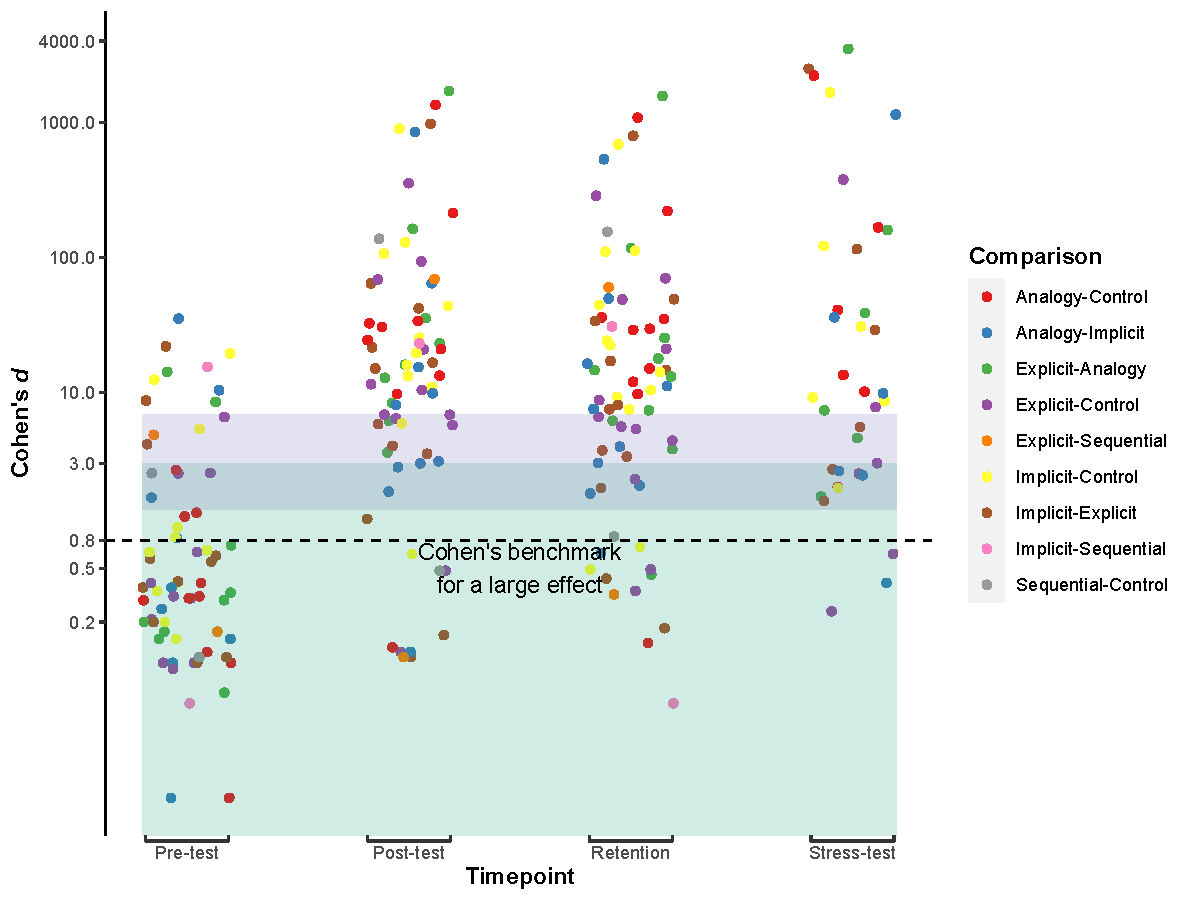
\includegraphics[width=1\linewidth,height=1\textheight]{../../figs/fig1} 

}

\caption{Absolute Cohen's \(d\) estimates from Articles 1-4 plotted on a logarithmic scale. All pairwise comparisons have been included for all dependent measures in each experiment. The range of observed values from a simulation of 1,000,000 experiments with a true effect of \(d\) = .8 is illustrated by shaded green and blue regions of the figure, reaching a maximum value of \(d\) = 2.97. The range of observed values from a simulation of 1,000,000 experiments with a true effect of \(d\) = 3 is illustrated by the shaded purple and blue regions of the figure, reaching a maximum value of \(d\) = 6.6.}\label{fig:fig1}
\end{figure}

In the context of the maximum values observed in our simulations, all five articles in question reported implausibly large effect sizes. In Article 1, the smallest pre-test difference for reaction time was \emph{d} = 1.29 and the largest pre-test difference was \emph{d} = 35.32---although none of the groups were reported as significantly different in the article. The smallest post-intervention effect at any of the three time points was \emph{d} = 286.42, while the largest effect was \emph{d} = 3504.86. A similar picture emerges when analyzing the accuracy data. All the pre-test differences were improbably large (all \emph{d}'s \(\geq\) 2.52) despite being reported as not significantly different in the articles. Ten of the pairwise comparisons resulted in \emph{d}'s \(\geq\) 100 following treatment with the independent variables. The motor component data revealed post-treatment effect sizes ranging from \emph{d} = 1.16 to \emph{d} = 13.5.

In Article 2, post-intervention motor performance effect sizes ranged from \emph{d} = 3.1 to \emph{d} = 20.95. Similarly, post-intervention self-efficacy effect sizes ranged from \emph{d} = 1.79 to \emph{d} = 44.46. Likewise, in Article 3 post-intervention reaction time effect sizes ranged from \emph{d} = 2.28 to \emph{d} = 35.97. Continuing this pattern, post-intervention response accuracy effect sizes ranged from \emph{d} = 5.84 to \emph{d} = 29.7.

In Article 4, many response accuracy effect sizes were implausibly large beginning at pre-test, wherein effects ranged from \emph{d} = 2.53 to \emph{d} = 15.50. Nevertheless, all pre-test comparisons were reported as non-significant. Following intervention, the effect sizes ranged from \emph{d} = 23.13 to \emph{d} = 155.08. Relative to other reported effect sizes, those reported for reaction time were not implausibly large at any time point, ranging from \emph{d} = 0 to \emph{d} = .86. However, the authors reported an implausibly large effect size, \(\eta^{2}\) = .94, for the 4 (Group) x 3 (Time) ANOVA. Further, despite only one pairwise comparison being statistically significant, all post-intervention comparisons were reported as being significant in the article.

In Article 5, the authors did not report means and standard deviations for most of the analyses. However, \(\eta^{2}\) effect sizes were reported and these ranged from \(\eta^{2}\) = .52 to \(\eta^{2}\) = .98. These effect sizes are discussed further below. All the post-intervention effects reviewed above were directionally consistent with the researchers' expectations. The sometimes implausibly large pre-test effects were not expected, but also were not reported as significant.

\hypertarget{impossible-data-and-granularity-analysis}{%
\subsection{Impossible Data and Granularity Analysis}\label{impossible-data-and-granularity-analysis}}

In Article 1, the Competitive State Anxiety Inventory-2 was used to assess the level of cognitive and somatic stress experienced by participants. Responses were measured on a Likert scale ranging from 1 to 4 with the data appearing to represent the average response per item. At each of the three low-stress time points, the means reported for all four groups ranged from 1.02 to 1.09. During the high-stress time point, the means ranged from 3.95 to 4.09. The means for two groups were reported as greater than 4, which is not possible given the maximum score on the Competitive State Anxiety Inventory-2 is 4.

In Article 2, participants were asked to receive a served volleyball and pass it to a target consisting of three concentric circles. Motor performance was measured based on where the pass landed, with three points awarded for a pass to the central circle on the target, two points for the middle circle, one point for the outermost circle, and zero points for a pass that missed the target.\footnote{Independent of the issues we have raised, this approach to measuring motor performance has been shown to be inappropriate and flawed for this type of task (see Fischman, 2015; Hancock, Butler, \& Fischman, 1995; Reeve, Fischman, Christina, \& Cauraugh, 1994 for discussions).} Results were presented as average performance per trial and the analogy group was reported to have a mean score of 3.00 at retention (a perfect score) but with a standard deviation of .09. The perfect score was not a rounding error because the same group was reported to have a mean score of 2.99 with a standard deviation of .11 on the post-test. These data are not possible.

Articles 1, 4, and 5 reported the means and standard deviations for the number of explicit rules recalled by participants following the intervention phase. As a single item analysis of integers these results were suitable for a GRIMMER analysis. In Article 1, the mean and standard deviation pairs were GRIMMER inconsistent for all four groups. In Article 4, the mean and standard deviation pair was GRIMMER consistent for the explicit rules group (\emph{M} = 4.8, \emph{SD} = 1.78). The mean and standard deviation pairs for the remaining three groups were GRIMMER inconsistent. In Article 5, the mean and standard deviation pairs were GRIMMER consistent for three of the four groups if the standard deviations were calculated for the population rather than the sample. For two of the groups, however, they were consistent regardless of which method of calculating the standard deviation was used. However, the results for the explicit group were GRIMMER inconsistent (\emph{M} = 4.8, \emph{SD} = 1.78).\footnote{You may have noticed that the same mean and standard deviation pairing (\emph{M} = 4.8, \emph{SD} = 1.78) was classified as GRIMMER inconsistent for one paper and consistent for the other. This is because of sample size differences (\emph{n} = 20 for the consistent result and \emph{n} = 12 for the inconsistent one).}

\hypertarget{eta-squared-eta2-1}{%
\subsection{\texorpdfstring{Eta-squared (\(\eta^{2}\))}{Eta-squared (\textbackslash eta\^{}\{2\})}}\label{eta-squared-eta2-1}}

Eta-squared (\(\eta^{2}\)) is calculated by dividing the sum of squares for the effect by the total sum of squares. It can be interpreted as analogous to \(R^{2}\) as it represents the total variation in the dependent measure that can be explained by a given main effect or interaction in an ANOVA (Lakens, 2013). Benchmarks have been suggested for small, medium, and large effect sizes as \(\eta^{2}\) = .01, .06, and .14, respectively (Cohen, 1988). Importantly, if a main effect of instruction-type results in \(\eta^{2}\) = .99, as was commonly reported in the target articles, this suggests that 99\% of the total variability in the outcome measure can be explained by group assignment alone. Such a result is implausible.

Article 1 did not report \(\eta^{2}\) values but had the largest pairwise effects and \emph{F}-statistics of the five articles in question. Article 2 reported \(\eta^{2}\) = .994, \(\eta^{2}\) = .996, and \(\eta^{2}\) = .996 for the Time, Group, and Time x Group effects on motor performance, respectively. Similarly, variance explained on the self-efficacy measure was \(\eta^{2}\) = .995, \(\eta^{2}\) = .994, \(\eta^{2}\) = .997 for the Time, Group, and Time x Group effects, respectively. Article 3 also reported \(\eta^{2}\) = .99 for all three effects on both response time and response accuracy measures.

Article 4 reported \(\eta^{2}\) = 1.0 for the main effect of Time and the Time x Group interaction, as well as \(\eta^{2}\) = .95 for the main effect of Group on the response time measure. Interestingly, the Time x Group interaction had the smallest reported significant \emph{F}-statistic among the five articles in question. With respect to response accuracy, the reported effects were \(\eta^{2}\) = .98, \(\eta^{2}\) = .94, \(\eta^{2}\) = .93 for the Time, Group, and Time x Group analyses, respectively. Article 5 reported \(\eta^{2}\) = .66, \(\eta^{2}\) = .52, \(\eta^{2}\) = .72 for the Time, Group, and Time x Group analyses, respectively.

\hypertarget{other-oddities}{%
\subsection{Other Oddities}\label{other-oddities}}

Although the means and standard deviations for the explicit rules analysis were only reported in three of the articles in question, analyses were reported in Articles 1, 3, 4, and 5. The reported test statistic in these four articles was \emph{F} = 52.67, albeit with different degrees of freedom in Article 5 that reflected the different sample size in this experiment (48 versus 60 in Articles 1, 3, and 4). Articles 1-3 were published over a span of 6 years with reported samples sizes of 60 in Articles 1 and 3, and 80 in Article 2. Yet, the authors report identical means and standard deviations for the age of their participants in these three articles (see Table \ref{tab:table1}). We assumed that each article was based on different samples as none of the articles mentioned using any previously published data.

\hypertarget{discussion}{%
\section{Discussion}\label{discussion}}

We have reviewed concerning data irregularities spanning five articles investigating implicit motor and perceptual learning (Lola \& Tzetzis, 2020, 2021; Lola et al., 2012; Tzetzis \& Lola, 2010, 2015). These data irregularities include implausibly large effect sizes for pairwise comparisons and impossible descriptive statistics---both of which have been acknowledged by the authors as misprints due to an outsourcing of table formatting (A. Lola, personal communication, April 22, 2021). Further, the reported test statistics and associated \(\eta^{2}\) values are also implausibly large, which is inconsistent with the authors' claim that the results and discussions remain valid despite these aforementioned typographic errors in the tables. Considering these findings, the conclusions from these articles are not reliable.

It is noteworthy that the results reported in each of these articles perfectly reflect the authors' expectations. Indeed, our attention was drawn to these articles after the Lola and Tzetzis (2021) paper was shared on Twitter (Gray, 2021); possibly because the results appeared to be exemplary. Although these errors seem unlikely to have aligned with expectations by chance alone, our exposure to them occurred after they had been selected for publication. We cannot rule out that these papers were selected for publication because of exemplary results and happened to have errors, and this selection caused those errors to correlate with the authors' expectations.

Other irregularities, such as a repeating \emph{F}-statistic for all four analyses of explicit rules and the recurring age of participants, potentially reflect sloppiness more than expectation. Indeed, the authors have already admitted that some values reported in their tables were in error, and it seems errors occurred in each of the articles we have reviewed. These errors were pervasive and appear to have substantially affected the conclusions of the articles in question. At a minimum, the consistent reporting errors across these five articles seem to reflect excessive carelessness throughout the publication process. Even if the authors offer corrections, which they have suggested they intend to do\footnote{As of today's date (2021-09-11), there is no indication that such corrective actions have been taken by the authors.}, many in the research community may find it difficult to trust any of these results.

\hypertarget{acknowledgements}{%
\section{Acknowledgements}\label{acknowledgements}}

We would like to thank Abbey Corson for her help with data extraction from the target articles.

\hypertarget{data-materials-and-code-availability}{%
\section{Data, materials, and code availability}\label{data-materials-and-code-availability}}

\label{sec:sharing} All material, data, and scripts to reproduce our analyses and figure can be accessed here: \url{https://osf.io/raz6q/}.

\hypertarget{r-packages-used-in-this-project}{%
\section{R packages used in this project}\label{r-packages-used-in-this-project}}

R (Version 4.1.1; R Core Team, 2021) and the R-packages \emph{compute.es} (Version 0.2.5; Re, 2013), \emph{daff} (Fitzpatrick, de Jonge, \& Warnes, 2019), \emph{gridGraphics} (Murrell \& Wen, 2020), \emph{kableExtra} (Version 1.3.4; Zhu, 2021), \emph{lemon} (Version 0.4.5; Edwards, 2020), \emph{lsr} (Navarro, 2015), \emph{papaja} (Version 0.1.0.9997; Aust \& Barth, 2020), \emph{RColorBrewer} (Version 1.1.2; Neuwirth, 2014), \emph{scales} (Version 1.1.1; Wickham \& Seidel, 2020), and \emph{tidyverse} (Version 1.3.1; Wickham et al., 2019).

\hypertarget{conflict-of-interest}{%
\section{Conflict of interest}\label{conflict-of-interest}}

The authors declare no competing interests.

\hypertarget{references}{%
\section{References}\label{references}}

\begingroup
\setlength{\parindent}{-0.5in}
\setlength{\leftskip}{0.5in}

\endgroup

\hypertarget{refs}{}
\begin{CSLReferences}{1}{0}
\leavevmode\vadjust pre{\hypertarget{ref-anaya2016}{}}%
Anaya, J. (2016). \emph{The GRIMMER test: A method for testing the validity of reported measures of variability}. \url{https://doi.org/10.7287/peerj.preprints.2400v1}

\leavevmode\vadjust pre{\hypertarget{ref-R-papaja}{}}%
Aust, F., \& Barth, M. (2020). \emph{{papaja}: {Create} {APA} manuscripts with {R Markdown}}. Retrieved from \url{https://github.com/crsh/papaja}

\leavevmode\vadjust pre{\hypertarget{ref-bakker2011}{}}%
Bakker, M., \& Wicherts, J. M. (2011). The (mis)reporting of statistical results in psychology journals. \emph{Behavior Research Methods}, \emph{43}(3), 666--678. \url{https://doi.org/10.3758/s13428-011-0089-5}

\leavevmode\vadjust pre{\hypertarget{ref-brown2017}{}}%
Brown, N. J. L., \& Heathers, J. A. J. (2017). The GRIM Test: A Simple Technique Detects Numerous Anomalies in the Reporting of Results in Psychology. \emph{Social Psychological and Personality Science}, \emph{8}(4), 363--369. \url{https://doi.org/10.1177/1948550616673876}

\leavevmode\vadjust pre{\hypertarget{ref-cohen1962}{}}%
Cohen, J. (1962). The statistical power of abnormal-social psychological research: a review. \emph{Journal of Abnormal and Social Psychology}, \emph{65}, 145--153. \url{https://doi.org/10.1037/h0045186}

\leavevmode\vadjust pre{\hypertarget{ref-cohen1988}{}}%
Cohen, J. (1988). \emph{Statistical power analysis for the behavioral sciences} (2nd ed.). New York: Routledge. \url{https://doi.org/10.4324/9780203771587}

\leavevmode\vadjust pre{\hypertarget{ref-correll2020}{}}%
Correll, J., Mellinger, C., McClelland, G. H., \& Judd, C. M. (2020). Avoid cohen{'}s {`}small{'}, {`}medium{'}, and {`}large{'} for power analysis. \emph{Trends in Cognitive Sciences}, \emph{24}(3), 200--207. \url{https://doi.org/10.1016/j.tics.2019.12.009}

\leavevmode\vadjust pre{\hypertarget{ref-R-lemon}{}}%
Edwards, S. M. (2020). \emph{Lemon: Freshing up your 'ggplot2' plots}. Retrieved from \url{https://CRAN.R-project.org/package=lemon}

\leavevmode\vadjust pre{\hypertarget{ref-field2016}{}}%
Field, A. P. (2016). \emph{An adventure in statistics: The reality enigma}.

\leavevmode\vadjust pre{\hypertarget{ref-fischman2015}{}}%
Fischman, M. G. (2015). On the continuing problem of inappropriate learning measures: Comment on Wulf et al. (2014) and Wulf et al. (2015). \emph{Human Movement Science}, \emph{42}, 225--231. \url{https://doi.org/10.1016/j.humov.2015.05.011}

\leavevmode\vadjust pre{\hypertarget{ref-R-daff}{}}%
Fitzpatrick, P., de Jonge, E., \& Warnes, G. R. (2019). \emph{Daff: Diff, patch and merge for data.frames}. Retrieved from \url{https://CRAN.R-project.org/package=daff}

\leavevmode\vadjust pre{\hypertarget{ref-gray2021}{}}%
Gray, R. {[}@ShakeyWaits{]}. (2021). \emph{The effect of explicit, implicit and analogy instruction on decision making skill for novices, under stress}. {[}Tweet; Thumbnail link to article{]}. Twitter. \url{https://twitter.com/ShakeyWaits/status/1359501377073012736}.

\leavevmode\vadjust pre{\hypertarget{ref-hancock1995}{}}%
Hancock, G. R., Butler, M. S., \& Fischman, M. G. (1995). On the problem of two-dimensional error scores: Measures and analyses of accuracy, bias, and consistency. \emph{Journal of Motor Behavior}, \emph{27}(3), 241--250. \url{https://doi.org/10.1080/00222895.1995.9941714}

\leavevmode\vadjust pre{\hypertarget{ref-lakens2013}{}}%
Lakens, D. (2013). Calculating and reporting effect sizes to facilitate cumulative science: A practical primer for t-tests and ANOVAs. \emph{Frontiers in Psychology}, \emph{4}. \url{https://doi.org/10.3389/fpsyg.2013.00863}

\leavevmode\vadjust pre{\hypertarget{ref-lola2020}{}}%
Lola, A. C., \& Tzetzis, G. C. (2020). Analogy versus explicit and implicit learning of a volleyball skill for novices: The effect on motor performance and self-efficacy. \emph{Journal of Physical Education and Sport}, \emph{20}(5), 2478--2486. Retrieved from \url{https://www.cabdirect.org/cabdirect/abstract/20203562097}

\leavevmode\vadjust pre{\hypertarget{ref-lola2021}{}}%
Lola, A. C., \& Tzetzis, G. C. (2021). The effect of explicit, implicit and analogy instruction on decision making skill for novices, under stress. \emph{International Journal of Sport and Exercise Psychology}, \emph{0}(0), 1--21. \url{https://doi.org/10.1080/1612197X.2021.1877325}

\leavevmode\vadjust pre{\hypertarget{ref-lola2012}{}}%
Lola, A. C., Tzetzis, G. C., \& Zetou, H. (2012). The Effect of Implicit and Explicit Practice in the Development of Decision Making in Volleyball Serving. \emph{Perceptual and Motor Skills}, \emph{114}(2), 665--678. \url{https://doi.org/10.2466/05.23.25.PMS.114.2.665-678}

\leavevmode\vadjust pre{\hypertarget{ref-lovakov2021}{}}%
Lovakov, A., \& Agadullina, E. R. (2021). Empirically derived guidelines for effect size interpretation in social psychology. \emph{European Journal of Social Psychology}, \emph{00}, 1--20. \url{https://doi.org/10.1002/ejsp.2752}

\leavevmode\vadjust pre{\hypertarget{ref-munafo2017}{}}%
Munafò, M. R., Nosek, B. A., Bishop, D. V. M., Button, K. S., Chambers, C. D., Percie du Sert, N., \ldots{} Ioannidis, J. P. A. (2017). A manifesto for reproducible science. \emph{Nature Human Behaviour}, \emph{1}(1), 1--9. \url{https://doi.org/10.1038/s41562-016-0021}

\leavevmode\vadjust pre{\hypertarget{ref-R-gridGraphics}{}}%
Murrell, P., \& Wen, Z. (2020). \emph{gridGraphics: Redraw base graphics using 'grid' graphics}. Retrieved from \url{https://CRAN.R-project.org/package=gridGraphics}

\leavevmode\vadjust pre{\hypertarget{ref-R-lsr}{}}%
Navarro, D. (2015). \emph{Learning statistics with r: A tutorial for psychology students and other beginners. (Version 0.5)}. Adelaide, Australia: University of Adelaide. Retrieved from \url{http://ua.edu.au/ccs/teaching/lsr}

\leavevmode\vadjust pre{\hypertarget{ref-R-RColorBrewer}{}}%
Neuwirth, E. (2014). \emph{RColorBrewer: ColorBrewer palettes}. Retrieved from \url{https://CRAN.R-project.org/package=RColorBrewer}

\leavevmode\vadjust pre{\hypertarget{ref-nuijten2016}{}}%
Nuijten, M. B., Hartgerink, C. H. J., van Assen, M. A. L. M., Epskamp, S., \& Wicherts, J. M. (2016). The prevalence of statistical reporting errors in psychology (1985{\textendash}2013). \emph{Behavior Research Methods}, \emph{48}(4), 1205--1226. \url{https://doi.org/10.3758/s13428-015-0664-2}

\leavevmode\vadjust pre{\hypertarget{ref-R-base}{}}%
R Core Team. (2021). \emph{R: A language and environment for statistical computing}. Vienna, Austria: R Foundation for Statistical Computing. Retrieved from \url{https://www.R-project.org/}

\leavevmode\vadjust pre{\hypertarget{ref-R-compute.es}{}}%
Re, A. C. D. (2013). Compute.es: Compute effect sizes. In \emph{R Package}. Retrieved from \url{https://cran.r-project.org/package=compute.es}

\leavevmode\vadjust pre{\hypertarget{ref-reeve1994}{}}%
Reeve, T. G., Fischman, M. G., Christina, R. W., \& Cauraugh, J. H. (1994). Using one-dimensional task error measures to assess performance on two-dimensional tasks: Comment on 'attentional control, distractors, and motor performance'. \emph{Human Performance}, \emph{7}(4), 315--319. \url{https://doi.org/10.1207/s15327043hup0704_6}

\leavevmode\vadjust pre{\hypertarget{ref-thompson2007}{}}%
Thompson, B. (2007). Effect sizes, confidence intervals, and confidence intervals for effect sizes. \emph{Psychology in the Schools}, \emph{44}(5), 423--432. \url{https://doi.org/10.1002/pits.20234}

\leavevmode\vadjust pre{\hypertarget{ref-tsorbatzoudis1998}{}}%
Tsorbatzoudis, H., Barkoukis, V., Kaissidis-Rodafinos, A., \& Grouios, G. (1998). A test of the reliability and factorial validity of the greek version of the CSAI-2. \emph{Research Quarterly for Exercise and Sport}, \emph{69}(4), 416--419. \url{https://doi.org/10.1080/02701367.1998.10607717}

\leavevmode\vadjust pre{\hypertarget{ref-tzetzis2010}{}}%
Tzetzis, G. C., \& Lola, A. C. (2010). The role of implicit, explicit instruction and their combination in learning anticipation skill under normal and stress conditions. \emph{International Journal of Sport Sciences and Physical Education}, \emph{1}, 54--59.

\leavevmode\vadjust pre{\hypertarget{ref-tzetzis2015}{}}%
Tzetzis, G. C., \& Lola, A. C. (2015). The effect of analogy, implicit, and explicit learning on anticipation in volleyball serving. \emph{International Journal of Sport Psychology}, \emph{46}(2), 152--166. \url{https://doi.org/10.7352/IJSP.2015.46.152}

\leavevmode\vadjust pre{\hypertarget{ref-R-tidyverse}{}}%
Wickham, H., Averick, M., Bryan, J., Chang, W., McGowan, L. D., François, R., \ldots{} Yutani, H. (2019). Welcome to the {tidyverse}. \emph{Journal of Open Source Software}, \emph{4}(43), 1686. \url{https://doi.org/10.21105/joss.01686}

\leavevmode\vadjust pre{\hypertarget{ref-R-scales}{}}%
Wickham, H., \& Seidel, D. (2020). \emph{Scales: Scale functions for visualization}. Retrieved from \url{https://CRAN.R-project.org/package=scales}

\leavevmode\vadjust pre{\hypertarget{ref-R-kableExtra}{}}%
Zhu, H. (2021). \emph{kableExtra: Construct complex table with 'kable' and pipe syntax}. Retrieved from \url{https://CRAN.R-project.org/package=kableExtra}

\end{CSLReferences}


\end{document}
